\documentclass{article}

% Language and font encodings
\usepackage[english]{babel}
\usepackage[utf8x]{inputenc}
\usepackage[T1]{fontenc}
\usepackage{verbatim} % multiline comments

% Sets page size and margins
\usepackage[a4paper,top=3cm,bottom=2cm,left=3cm,right=3cm,marginparwidth=1.75cm]{geometry}

% Useful packages
\usepackage{amsmath}
\usepackage{float}
\usepackage{rotating}
\usepackage{booktabs}
\usepackage{graphicx}
\usepackage[colorinlistoftodos]{todonotes}
\usepackage[colorlinks=true, allcolors=blue]{hyperref}
\usepackage[round]{natbib}
\usepackage[switch]{lineno} % line numbers
\usepackage{longtable}
\usepackage{multirow}

% Supplementary Materials
\newcommand{\beginsupplement}{
	\setcounter{table}{0}
    \renewcommand{\thetable}{S\arabic{table}}
    \setcounter{figure}{0}
    \renewcommand{\thefigure}{S\arabic{figure}}
}

\title{Dewlap color variation in \textit{Anolis sagrei} is maintained among habitats within islands of the West Indies}

\author{
	
    \textsc{Rapha\"{e}l Scherrer$^{1,3}$ \thanks{Corresponding author: r.scherrer@rug.nl}, Colin M. Donihue$^{1,4}$, }\\
	\textsc{R. Graham Reynolds$^2$, Jonathan B. Losos$^{1,4}$ and Anthony J. Geneva$^{1,5}$} \\[1ex]
	
	\normalsize $^1$ Department of Organismic and Evolutionary Biology and Museum of Comparative Zoology \\ \normalsize Harvard University, Cambridge, MA, USA \\
	\normalsize $^2$ Department of Biology, University of North Carolina Asheville, Asheville, NC, USA\\ 
	\normalsize $^3$ Current address: Groningen Institute for Evolutionary Life Sciences,\\
	\normalsize University of Groningen, Groningen, The Netherlands\\
	\normalsize $^4$ Current address: Department of Biology, Washington University, St. Louis, MO, USA\\
	\normalsize $^5$ Current address: Department of Biology, Center for Computational and Integrative Biology,\\ \normalsize Rutgers University--Camden, Camden, NJ, USA
	
}

\date{} % Leave empty to omit a date

\begin{document}
	
	\linenumbers
	
	\maketitle

	\begin{abstract}
    	Animal signals evolve in an ecological context. Moreover, locally adapting animal sexual signals can be especially important for initiating or reinforcing reproductive isolation during the early stages of speciation. Dewlap color in \textit{Anolis} lizards can be highly variable between populations in relation to both biotic and abiotic adaptive drivers, albeit at relatively large geographical scales. Here, we investigated local adaptation of the dewlap across habitat-types at a small spatial scale, as this may give an indication of how conditions for the early stages of speciation may be met. We explored variation in dewlap coloration in the most widespread species of anole, \textit{Anolis sagrei}, across three characteristic habitats spanning the Bahamas and the Cayman Islands. Using reflectance spectrometry as well as supervised machine learning, we found some consistent differences in spectral properties of the dewlap between habitats within small islands. Passive divergence in dewlap phenotype associated with isolation-by-distance did not explain our results. Instead, the observed patterns in dewlap coloration are more consistent with an adaptive explanation in these \textit{A. sagrei} populations, as one would otherwise expect differences within islands to be erased by gene flow at such small geographical scales. Although these habitat-specific dewlap differences vary in magnitude and direction across islands, and islands themselves differ substantially, we found a suite of consistent archipelago-wide differences between habitat types, suggesting parallel responses to similar selective pressures. While at present, populations from these different habitats probably experience too much gene flow to follow distinct evolutionary lineages, should additional barriers arise between habitat-specific populations, the observed disruptive selection on dewlap coloration may facilitate ecological speciation.
	\end{abstract}

	\textbf{Keywords} --- reflectance, adaptation, sexual signal, machine learning, polymorphism

	\section*{Introduction}
	
	The staggering diversity of animal communication signals has long been of interest to evolutionary biologists. Animals use chemical, mechanical, electromagnetic, and visual signals to communicate in a wide variety of contexts, including, competition for mates, species recognition, aposematism, and cooperation \citep{Bradbury2011}. A primary evolutionary factor shaping communication signals is the sensory system and behavior of recipients (the sensory drive hypothesis; \citealt{Endler1988,Endler1992,Endler1998}). Over the past decades, scientists have established that signals evolve in an ecological context and are dependent on environmental conditions \citep{Endler1992,Endler1993,Endler1993a}. Just as different habitats may favor different combinations of ecomorphological traits to maximize performance and fitness \citep{Arnold1983}, they may also shape different forms of a signal, so as to maximize its transmission and detection (e.g. \citealt{Seehausen1997}), or reduce its detection by unintended recipients such as predators \citep{Endler1984,Endler1990,Endler1991,Halfwerk2014}. This selective pressure may drive the local adaptation of communication signals.\\

One potential barrier to the maintenance of localized signal divergence is the homogenizing effect of gene flow. Population genetics theory suggests that gene flow may counteract local adaptation between localities and prevent divergence altogether, especially at small spatial scales, because of the inflow of maladapted alleles or because of the breaking of linkage between coevolving loci \citep{Felsenstein1976, Garcia-Ramos1997, Dieckmann1999, Lenormand2002, Hendry2007}. This genetic homogenization has been confirmed empirically in systems such as stick insects \citep{Nosil2004} and stickleback \citep{Hendry2007a}. Yet, examples of microgeographic adaptation, i.e. adaptation at smaller scales than the range of dispersal, exist, highlighting the potential of some organisms to respond to selection in the face of gene flow (see \citealt{Richardson2014} and references therein). Examples include small scale adaptation in fragmented areas in Australian fruit flies \citep{Willi2012}, and local adaptation to predation pressure in North American salamanders \citep{Richardson2013}. Therefore, despite evidence that local adaptation may be particularly difficult at small spatial scales where gene flow tends to cause adjoining populations to remain genetically homogeneous, the potential adaptive response of species traits, in particular communication signals, to localized differences in habitats remains relatively unknown \citep{Richardson2014}. Lizards of the neotropical genus \textit{Anolis} are an excellent group for studying the eco-evolutionary dynamics of local adaptation and natural selection \citep{Losos2009}. A particularly conspicuous trait of anoles is their dewlap, an extensible flap of skin that is typically sexually dimorphic and used as a communication signal in courtship \citep{Sigmund1983, Driessens2014, Driessens2015} and territorial displays \citep{Losos1985, Macedonia1994, Macedonia2013} as well as in predator deterrence \citep{Leal1995, Leal1997, Leal1997a}. Dewlap characteristics vary widely among the approximately $400$ species of the genus \citep{Nicholson2007}. Interspecific variation in dewlap coloration is implicated in species recognition \citep{Rand1970, Williams1969, Williams1977, Losos1985, Macedonia1994, Fleishman2000, Macedonia2013}, and this function could have had a role in initiating or reinforcing reproductive isolation during speciation \citep{Lambert2013, Geneva2015, Ng2017}.\\

Within species, studies have shown a link between variation in dewlap coloration and differences in habitats or climatic conditions \citep{Macedonia2001, Leal2002, Thorpe2002, Thorpe2002a, Leal2004, Vanhooydonck2009, Ng2012, Ng2013, Ng2016, Vanhooydonck2009, Driessens2017}. Some studies suggest that those differences may be adaptive and that dewlaps may have evolved to maximize detectability given local light conditions \citep{Fleishman2001, Leal2002, Leal2004}. Although this claim is further supported by recent findings that dewlap colors are perceived differently under different levels of shading \citep{Fleishman2020}, other studies found conflicting patterns of between-habitat variation that did not support the sensory drive hypothesis \citep{Fleishman2009, Ng2012, Macedonia2014}.\\ 

Previous studies investigating variation in anole dewlaps compared populations at relatively large geographical scales, e.g. between islands \citep{Vanhooydonck2009, Driessens2017} or within large islands such as Puerto Rico \citep{Leal2004} or Hispaniola \citep{Ng2012, Ng2016}. These large scales and marine barriers should reduce gene flow \citep{Ng2011, Lambert2013, Richardson2014, Ng2017}. That said, examples do exist of divergence in dewlap coloration at smaller scales or between populations with high degrees of gene flow \citep{Thorpe2002, Thorpe2002a, Stapley2011, Ng2016}.\\

\textit{Anolis sagrei} is widespread across islands of the West Indies \citep{Reynolds2020}. It has been the subject of numerous studies concerning local adaptation \citep{Losos1994, Losos1997a, Losos2001, Kolbe2012}, biological invasion \citep{Kolbe2008}, and sexual selection \citep{Tokarz2002, Tokarz2005, Tokarz2006, Driessens2014, Steffen2014, Driessens2015} among many other topics. Between-island variation in the mainly orange-red color of its dewlap was shown to be better explained by climatic variables \textcolor{olive}{such as annual precipitation and solar radiation (proposed to affect the average vegetation type on each island and among other things, its ambient light environment, \citealt{Driessens2017})},  than by proxies for biotic factors such as sexual selection or predation pressure \citep{Vanhooydonck2009, Baeckens2018}. How intra-island differences in habitat may contribute to the diversity of dewlap coloration, however, remains unexplored, and may reveal new insights into the scale of local differentiation despite gene flow.\\

Here, we analyzed the color characteristics of \textit{A. sagrei} dewlaps within nine islands in the Bahamas and Cayman Islands. These island systems presently, if not historically, comprise relatively small islands, with no major geographic barriers within islands limiting dispersal for this species. These islands all share three characteristic native West Indian small-island habitat-types -- beach scrub bush, closed-canopy primary coppice forest, and mangrove forest -- that are often spatially intermingled. These habitats contrast in environmental parameters including vegetation community, light irradiance, humidity, and temperature \citep{Howard1950, Schoener1968}. The Cayman Islands and the Bahamas have been colonized independently by \textit{A. sagrei} from Cuba (\citealt{vandeSchoot2016} unpublished thesis; \citealt{Reynolds2020}), such that these archipelagos constitute an ideal suite of natural replicates to explore within-island dewlap diversity across multiple islands.\\

Our sampling design included sites in close proximity; the median distance between two sites within an island was $11.2$km. \textcolor{olive}{While this species has traditionally been considered territorial, recent study reveals that they are polygynandrous and that gene flow is not impeded by territorial-like behaviors exibited by some males (Kamath and Losos 2018).} Combining reflectance spectrometry and supervised machine learning, we tested for divergence in dewlap phenotype between habitats within islands and between islands across part of the range of \textit{A. sagrei}. We predicted that if light conditions in the environment indeed drive color evolution, dewlaps should be most similar between beach scrub and mangrove forest, which both have high levels of light irradiance, compared to the darker, closed-canopy coppice forest. If detectability is maximized given the local conditions, we expected darker and more contrasting dewlaps in high irradiance habitats. Finally, if habitat characteristics are strong determinants of dewlap color variation, similar patterns should be observed across multiple islands \citep{Harvey1991, Losos2011}.

	\pagebreak
	
	\section*{Methods}

	\subsection*{Data collection}

We sampled 455 male \textit{A. sagrei} from seven islands in the Bahamas Archipelago -- Abaco, North Andros, South Andros, South Bimini, Eleuthera, Long Island, and Ragged Island -- and two in the Cayman Islands -- Cayman Brac and Little Cayman (Figure \ref{fig:maps}A). These islands were chosen to span the breadth of the West Indian range of \textit{A. sagrei}, because they have highly similar habitat types,  and because the \textit{A. sagrei} on each island group are derived from ancient and distinct colonization events from Cuba (i.e. relatively evolutionarily independent, \citealt{Reynolds2020}). Three habitats were sampled on each island based on characterizations by \citet{Howard1950} and \citet{Schoener1968}. Each habitat is clearly distinguishable by its dominant vegetation type --- xeric beach scrub (open, relatively dry habitat consisting of low vegetation or isolated trees), primary coppice forest (closed-canopy forest) and mangrove forest (wet coastal habitat with trees growing in brackish water and high light penetration, although lizards were sampled in dry soil areas). Sample sizes are given in Table \ref{tab:counts}. Our sampling design enabled us to test for differences between habitats at a coarse and fine geographical scale. The median distance between two localities within an island was $~8.5$km (Figure \ref{fig:maps}B), and 79.3\% of all pairwise distances within islands were less than $50$km. Additionally, there are no major barriers to dispersal (such as mountains or grassland) on any of the islands that we sampled.

\subsection*{Reflectance measurements}

We measured reflectance between 300nm and 700nm wavelength, a range from ultraviolet to red that encompasses the colors visible to most lizards and vertebrates in general \citep{Lazareva2012}. Measurements were taken with an Ocean Optics USB4000 spectrometer, a pulsed Xenon light source (PX-2, Ocean Optics, Largo, FL, USA) and a reflectance probe protected by a black anodized aluminum sheath. Measurements were taken with a 45-degree inclination to prevent specular reflection \citep{Endler1990}. The device was regularly standardized with a Spectralon white standard (Labsphere, North Sutton, NH, USA). Reflectance was measured at the center of the dewlap. Reflectance curves were smoothed using the R package pavo \citep{Maia2013} as well as with custom R functions, down to one reflectance value at each nanometer in wavelength from 300 to 700nm. 

\subsection*{Analysis}

We tested for detectable differences in dewlap coloration between populations from different habitats across islands by following an analytic pipeline in several steps. First, we used multivariate analyses of variance to assess the relative contributions of islands, habitats and habitat-by-island interactions on the partitioning of variation in color space. Second, and provided that habitat-by-island interactions were found, we investigated habitat-differences in dewlap color for each island separately using machine learning classification. Third, for each island where multivariate differences were detected using our machine learning pipeline, we used univariate analyses of variance to decompose the signal among the different dimensions of color space. Fourth, for each significant between-habitat variation found in univariate analyses, we used post-hoc tests to determine which habitats were responsible for the differences. Last, to get insights into the spatial scale of phenotypic variation, for each significant contrast between two habitats detected along a given dimension on a given island, we performed multiple pairwise Wilcoxon tests to assess differences in dewlap coloration among the sites involved in that significant contrast, and recorded the geographical distance between sites that were found significant. In parallel, we tested a possible effect of isolation-by-distance, an alternative cause of phenotypic divergence between localities, based on diffusion approximation and dispersal distance, irrespective of habitat types. We did so using a permutation test to assess the significance of the correlation between geographical distances and phenotypic distances among sites within each island.\\

All analyses in this study were performed in R 3.6.1 \citep{RCoreTeam2019}.

\subsubsection*{Dimensionality reduction}

Because neighboring wavelengths are highly collinear and redundant in reflectance, we reduced the dimensionality of the data using principal component analysis (PCA), as per \citet{Cuthill1999} and \citet{Leal2002}. We performed PCA on data from all islands combined, as well as on each island separately and systematically retained the first four principal components (PC), which together always explained more than $88.8\%$ of the variance across islands (Table \ref{tab:pcavariances}). PCs need not represent the same wavelengths across islands because they are fitted on different datasets. Nevertheless, PC1 was highly collinear with brightness for all islands (Figure \ref{fig:brightness}), while the other PCs captured the chromatic variation (i.e. irrespective of brightness) in dewlap color.

\subsubsection*{Among-island variance partitioning}

We performed a two-way nonparametric multivariate analysis of variance (PERMANOVA, \citealt{Anderson2001}, R package vegan, \citealt{Oksanen2019}) to identify differences in coloration between islands, habitats and habitats within islands, using principal components fitted on data from all islands together. We used a nonparametric test because although no multivariate outliers were detected based on the Mahalanobis distance, the assumption of multivariate normality was violated in several habitats on several islands (Henze-Zirkler's test, \citealt{Henze1990}, R package MVN, \citealt{Korkmaz2014}, $P < 0.05$, Table \ref{tab:multinorm}).

\subsubsection*{Within-island machine learning}

We performed a machine learning classification analysis on the first four principal components within each island separately, using random forests \citep{Breiman2001}. Random forests are a versatile, intuitive, and powerful algorithm commonly used in machine learning, using decision trees to predict the labels of particular observations based on their multivariate coordinates. These coordinates, or variables, are passed through a series of successive decision nodes, each examining a given variable of any given observation \citep{James2013}. The prediction for each observation is an aggregate over a large number of decision trees, each tree being trained on a subset of observations sampled with replacement from the dataset, and each tree being allowed to examine only a subset of the variables. This allows the random forest to overcome the individual errors of all trees in the predictions it makes.\\

To detect differences in dewlap coloration between habitats, we measured the success of random forests in reassigning individual lizards to their correct habitat of origin, based solely on their principal component scores. In machine learning, this so-called cross-validation procedure is typically done in two steps \citep{James2013}. First, a random forest is trained in recognizing features of dewlap coloration most associated with the different habitats, by being presented with multiple observations, making predictions about them, and updating its own decision rules based on whether the prediction deviates from the truth. Then, once trained, the patterns that the random forest has learned to recognize are tested by presenting new, previously unseen observations to the random forest, and measuring the proportion of correct predictions. This proportion, or success score, can then be statistically assessed against random guessing using a binomial test.\\

The cross-validation procedure requires that the data be split into a training set and a testing set. To remove any bias due to the set that is being sampled for training, it is common practice to use k-fold cross-validation \citep{James2013}, where the data are split into $k$ random bins and $k$ independent machines are trained, each taking one of the bins as a testing set and the rest for training, and where classification success is measured by summing all correct classifications from the $k$ machines.\\

Here, we used a k-fold cross-validation procedure with $k = 5$, where each training set consisted of 80\% of the data and the machine was tested on the remaining 20\%. Each training set was conditioned on containing at least five lizards from each of the three habitats. We also down-sampled the training set to the sample size of the least represented habitat, to ensure that the different habitats were equally represented. To further remove any bias due to the specific random split into the different bins, we replicated each k-fold cross-validation five times. We then averaged the five resulting confusion matrices across replicates, where each confusion matrix shows the number of lizards from each habitat reassigned into each habitat. For each island, we then used the average proportion of correctly reassigned lizards (i.e. the proportion of observations on the diagonal of the average confusion matrix) as an estimate of classification success. This score was tested against random guessing by comparing it to a binomial distribution with number of trials being the number of lizards on that island and success probability $1/3$, representing the rate of successful classification by chance when three habitats are involved.\\

We used the machine learning fitting functions in the R package rminer \citep{Cortez2020}, which calls random forest routines from the randomForest package (\citealt{Liaw2002}, implementation from the original random forest algorithm \citealp{Breiman2001}). For each random forest, we optimized the number of trees in the forest and the number of variables examined by each tree using the grid hyperparameter search procedure implemented in rminer, to choose between two numbers of trees (500 or 1,000) and four numbers of principal components examined per tree (1 to 4), using rminer's ordered holdout validation method with $2/3$ of the data used for training.\\

We validated the results of our analysis by using two other widely used machine learning classification methods: linear discriminant analysis and support vector machines \citep{Cristianini2000, James2013}, both accessible in rminer \citep{Cortez2020}.\\

To know which wavelengths were most used to assign data points to each habitat, we trained another set of random forests, this time directly on reflectance data (taken every 5nm from 300 to 700nm) instead of principal components. We recorded the relative importance of each wavelength for each habitat, as measured by the mean decrease in accuracy during wavelength permutation, implemented in the randomForest package \citep{Liaw2002}.

\subsubsection*{Univariate analyses}

For each island where significant differences in dewlap coloration were detected between habitats, we used multiple univariate analyses of variance (ANOVA) to identify possible principal components underlying the observed differences. We constructed our ANOVA models in two steps, as per \citet{Zuur2009}. In a first step, we accounted for heterogeneity of variances across groups by systematically comparing the goodness-of-fit of an ANOVA model estimated with ordinary least squares (OLS) with that of a model estimated with generalized least squares (GLS), which allowed one estimate of residual variance per habitat (using the R package nlme, \citealt{Pinheiro2000, Pinheiro2020}). Both models were fitted with restricted maximum likelihood (REML). Goodness-of-fit was estimated using Akaike's Information Criterion corrected for small sample sizes (AICc, R package MuMIn, \citealt{Barton2019}), and the estimation method yielding the lowest AICc was retained. In a second step, we re-fitted the retained model with maximum likelihood (ML) to test for the effect of habitat type using likelihood ratio tests (LRT) between a model including a habitat-term and a null model lacking the habitat-term.\\

We evaluated the normality of the standardized residuals (residuals divided by their standard error, which can differ among habitats in a GLS model) of each fitted ANOVA model using Shapiro-Wilk's test, with P-values adjusted for multiple testing using the Benjamini-Hochberg correction \citep{Benjamini1995}. In cases where significant deviations from normality were detected ($P_{adj} < 0.05$, Table \ref{tab:normality}) we performed Kruskal-Wallis's nonparametric test to back up the ANOVA results.\\

To know which habitat-populations were different from which in dewlap coloration, we performed different post-hoc multiple comparison tests (all implemented in the PMCMRplus package, \citealp{Pohlert2020}), depending on which assumptions were met. In cases where normality and homoscedasticity were met (i.e. OLS-ANOVA was the best fit), we used Tukey's honest significant difference test. When normality was met but not homoscedasticity (i.e. GLS-ANOVA was the best fit), we used Dunnett's T3 test. Finally, whenever we used Kruskal-Wallis's test because the ANOVA residuals were not normally distributed, we used Nemenyi's test for post-hoc comparisons.

\subsubsection*{Spatial autocorrelation}

We tested for within-island spatial autocorrelation between the geographical distances among sampling sites and their Euclidean distances in multivariate color space (mean PC1 to PC4 per site, Table \ref{tab:sites}), regardless of habitat type. For this, we performed Mantel's test (\citealt{Legendre2012}, R package vegan; \citealt{Oksanen2019}) on each island, using 999 permutations and geographical distances computed as geodesic distances from latitude and longitude data (R package geosphere, \citealt{Hijmans2019}).\\ 

\subsubsection*{Site differences}

In this study, we were interested in the minimum spatial scale at which significant differences between habitats could be detected within islands. We performed multiple pairwise nonparametric Wilcoxon-Mann-Whitney tests \citep{Hollander2013} to compare dewlap coloration between sites with different habitat types, for each pair of habitats and each variable where significant differences were detected with our analyses of variance. The P-values were adjusted using a Benjamini-Hochberg correction for multiple testing \citep{Benjamini1995}.

	\pagebreak
	
	\section*{Results}

	We tested for variation in \textit{A. sagrei} dewlap coloration between populations living in three characteristic habitat types across nine islands that span the West Indian range of the brown anole (beach scrub, primary coppice and mangroves). We found that most of the variation in coloration was partitioned between islands (two-way PERMANOVA, $F(df = 8) = 45.38$, $P = 0.001$, explained variance $R^2 = 41.4$\%). Nonetheless, we did find evidence for differences in dewlap coloration between habitat types, and those were mostly island-specific (habitat-by-island interaction term, $F(16) = 4.78$, $P = 0.001$, $R^2 = 8.7$\%), with a significant portion of the variation explained by an habitat effect across all islands, but this effect was relatively small ($F(2) = 4.46$, $P = 0.001$, $R^2 = 1$\%).\\

We subsequently tested for differences in dewlap coloration between habitat-populations within each island, using within-island principal component scores (to maximize the variation captured for each island, see Methods). Our within-island random forest classification analyses revealed detectable differences in dewlap coloration on seven out of the nine islands in our sample: Abaco, Bimini, Cayman Brac, Eleuthera, Little Cayman, Long Island, and North Andros. The accuracy of random forest classification exceeded random expectation more often than expected by chance for all these islands (Table \ref{tab:randomforests}). Accuracy was as high as 74.8\% for Cayman Brac. We obtained similar results using other machine learning approaches such as support vector machines (Table \ref{tab:ksvms}) and linear discriminant analysis (Table \ref{tab:ldas}). We describe in details the specific differences detected on each island in the Appendix, and focus here on the general patterns emerging from our data.\\

Overall, we found significant differences in dewlap coloration between populations that were often in close geographical proximity. On Bimini, notably, we found a significant difference between dewlaps from beach scrub and primary coppice forest, at a distance of a few hundred meters, making this contrast the smallest geographical scale at which differences in coloration were found in our study (Fig. \ref{fig:Bimini}). We also detected significant differences in dewlap coloration at distances below one kilometer on Abaco (Fig. \ref{fig:Abaco_supplement}G), and at distances between one and ten kilometers on Bimini (Fig. \ref{fig:Bimini}G), Cayman Brac (Fig. \ref{fig:CaymanBrac}G), Little Cayman (Fig. \ref{fig:LittleCayman}G), Long Island (Fig. \ref{fig:LongIsland}G) and North Andros (Fig. \ref{fig:NorthAndros}G).\\

We found evidence of spatial autocorrelation in dewlap coloration between the sites within islands for Abaco (Table \ref{tab:autocorrelation}), suggesting that populations from closer sites tend to have more similar dewlaps on this island than expected by chance. Abaco was the island we sampled at the largest scale, with some sites nearly a hundred kilometers away from each other (Fig. \ref{fig:Abaco}A). That said, some sites were also in close proximity, and significant differences in coloration were detected between habitats sometimes less than a kilometer away (Fig. \ref{fig:Abaco_supplement}G), suggesting that differences in dewlap coloration between distant sites may be partly attributable to isolation-by-distance, but this may not necessarily be the case for sites in close proximity. We did not find evidence for spatial autocorrelation on other islands than Abaco (although Eleuthera was nearly significant, Table \ref{tab:autocorrelation}).\\

A striking feature of our data was inconsistency in between-habitat differences among islands, in terms of which habitats differ from which, which dimensions of coloration were involved, and in which direction. For example, while on Cayman Brac the random forests could well distinguish between all three habitats (Fig. \ref{fig:CaymanBrac}D), on Abaco dewlaps from beach scrub and primary coppice were often mistaken, and on Bimini beach scrub dewlaps were more often classified into primary coppice or mangrove than into beach srub (Fig. \ref{fig:Bimini}D). In terms of variable importance, for multiple islands the random forests used information in the UV range to discriminate between at least some habitats, particularly on Abaco (Fig. \ref{fig:Abaco_supplement}F), Bimini (Fig. \ref{fig:Bimini}F), Cayman Brac (Fig. \ref{fig:CaymanBrac}F), Little Cayman (Fig. \ref{fig:LittleCayman}F) and Long Island (Fig. \ref{fig:LongIsland}F), but differences in UV reflectance involved different habitats and were in different directions among these islands.\\

	\pagebreak

	\section*{Discussion}

	Two main insights follow from our results. First, we detected significant differences in dewlap coloration between habitats within seven out of the nine islands investigated (excluding North Andros where the follow-up univariate analyses were not significant), suggesting a putatively high potential for local differentiation of dewlap coloration in \textit{Anolis sagrei}. Second, we found differences in coloration along different dimensions of color space, and in different directions, on different islands.\\

Detectable differences in dewlap color between populations are surprising, as habitats were often in close geographical proximity to each other (as close as a few hundred meters on Bimini and most of the time within ten kilometers)\sout{. Indeed, given that (1) the populations were continuously distributed between the habitats, (2) populations from different habitats were not monophyletic with respect to mitochondrial haplotypes (van de Schoot 2016 unpublished thesis), and (3) \textit{A. sagrei} is highly mobile (Kamath and Losos, 2018b), we would have expected more homogeneous distributions of color phenotypes within islands due to gene flow, with fewer differences between populations, especially those in close proximity.} \textcolor{olive}{, and we would have expected gene flow to cause a more homogeneous distribution of color phenotypes within islands. While little is known about the cruising range of individuals from our study populations (but see \citealt{Steinberg2017, Kamath2018} for other systems), \textit{A. sagrei} are polygynandrous (both males and females mate with multiple mates, \citealt{Kamath2017, Kamath2018a, Kamath2018}), thus offering opportunity for gene flow, especially given that lizards were distributed continuously and at high densities within the islands we sampled. Consistent with that, while populations from different islands were monophyletic, individuals within islands were not monophyletic with respect to habitat based on mitochondrial haplotypes (\citealt{vandeSchoot2016} unpublished thesis).}\\

Several scenarios could account for these findings. One explanation is an adaptive one: populations living in different habitats could be phenotypically adapted to their local environmental conditions. Given that the brightly colored dewlap of \textit{A. sagrei} is used as a communication signal, its color may be a target for selection if the transmission or perception of the signal differs from one habitat to another, for example because of differences in ambient light, according to the sensory-drive hypothesis \citep{Endler1988, Endler1992, Endler1998}. The sensory-drive hypothesis has been tested multiple times for dewlap coloration in \textit{Anolis} lizards, with mixed results. Some authors found support for it \citep{Leal2002, Leal2004}, while others found differences in dewlap coloration between habitats inconsistent with the sensory-drive hypothesis \citep{Fleishman2009, Ng2012}.\\

If our results were an example of sensory drive, we would have expected to see consistent differences between populations from different habitats across islands, given the apparent environmental consistency each of the three habitat types across the islands we sampled. In particular, we would have expected divergence in line with increased detectability given local light conditions, such as the high contrasts with background vegetation found in the UV range in \citet{Leal2002} and \citet{Leal2004}. We might also have expected mangrove and beach scrub lizards, both inhabiting areas with high light penetration, to have more similar dewlaps, and to differ significantly from lizards from the coppice habitat, where irradiance is low. Instead, we found inconsistencies in the way dewlap color differed between habitats across islands. While short-wavelengths (UV reflectance) were often involved in color differences, they were not involved on all islands where significant differences were detected. On some islands, other or additional variables differed, such as brightness, red reflectance or the reflectance at the ends of the spectrum visible to \textit{Anolis} lizards (UV and red, \citealt{Lazareva2012}) relative to intermediate wavelengths (blue-to-yellow). Similar portions of the spectrum were sometimes involved in opposite directions on different islands, such as on Abaco and Cayman Brac, where mangrove lizards had a higher UV-reflectance than beach scrub lizards on the former, but a lower UV-reflectance on the latter. Overall, the observed heterogeneity of divergence patterns across islands provides no support to a sensory-drive explanation.\\

It is presently not known if the reported differences in coloration have a genetic basis. Yet, we find it unlikely that these differences arose through phenotypic plasticity, as although the carotenoids that partly make up the red and orange colors of anole dewlaps must be found in the diet \citep{Goodwin1984, Hill2002, Hill2006}, studies testing the effect of carotenoid deprivation \citep{Steffen2010, Ng2013} and heritability \citep{Cox2017} of dewlap coloration in \textit{A. sagrei} and \textit{A. distichus} (another species with a carotenoid-based dewlap), found little support for phenotypic and developmental plasticity in dewlap coloration. One exception is a study demonstrating that lizards heavily parasitized by skin mites had duller dewlaps \citep{Cook2013}, but we found no sign of that in our study.\\

\sout{We found no evidence for a role of genetic drift in explaining the observed patterns either. First, \textit{A. sagrei} was distributed across the islands continuously, usually at relatively high population densities, rather than in small and isolated populations where drift might be expected to have a strong effect. Second, we found no evidence of isolation-by-distance except on Abaco, which was sampled at the largest geographical scale, with sites nearly a hundred kilometers apart from each other. Hence, while isolation-by-distance may explain long-range differences on this island, most of the differences among habitats across the rest of the sampling region are unlikely to be explained by genetic drift, as habitats were often in close proximity (less than 10km).}\\

\textcolor{olive}{Genetic drift could contribute to some of the observed variation. Indeed, while only Abaco showed significant patterns consistent with isolation-by-distance (which may emerge under limited dispersal and drift, \citealt{Wright1943, Kimura1964, Slatkin1987}), there may have been too few sites on most islands to conclusively detect it, and even then, the absence of detectable isolation-by-distance may not necessarily constitute evidence for the absence of drift. Besides, spatial autocorrelation was the strongest on islands sampled at the largest scales (e.g. some sites on Abaco were nearly 100km apart, and Eleuthera -- the second strongest signal, albeit nonsignificant -- had sites more than 30km apart), such that it is possible that neutral processes and/or dispersal limitations might contribute to shaping variation over long distances. That said, many significant differences were found between habitats in close proximity, contrary to what would be expected under isolation-by-distance, including on islands where spatial autocorrelation was detected. Moreover, \textit{A. sagrei} was distributed across the islands continuously, usually at relatively high population densities, rather than in small and isolated populations particularly prone to drift. Together with the fact that isolation-by-distance may not necessarily only emerge from drift (e.g. if there is a spatial environmental gradient), this indicates that genetic drift may have limited potential to explain the differences observed between habitats, at least at a local scale.}\\

In this study, we found larger differences among than within islands, a pattern already reported and linked to climatic conditions \citep{Driessens2017} and to densities of predators and of anole congeners \citep{Vanhooydonck2009, Baeckens2018}. Differences among habitats within islands, however, are still difficult to account for. Remaining hypotheses may include, for example, runaway sexual selection \textcolor{olive}{(i.e. arbitrary preferences of females for some colors over others, \citealt{Andersson1994})} \sout{arbitrarily} operating in different directions across islands, but no evidence so far suggests that dewlap is a target of mate choice in anoles \citep{Tokarz2002, Tokarz2005, Lailvaux2006, Nicholson2007}. Another hypothesis is that the different genetic constitutions of different islands, perhaps resulting from founder effects (the islands have been colonized independently, \citealt{vandeSchoot2016} unpubl.; \citealt{Driessens2017, Reynolds2020}), may have predisposed populations to adapt differently to similarly selective circumstances. Either way, new data would be needed to test these hypotheses. \textcolor{olive}{Visual modeling, for instance, would be a valuable follow-up analysis as it would indicate whether the differences we detected may be detectable by the organisms themselves (as has been done in \textit{Anolis} in \citealt{Leal2004, Fleishman2020}), but such approach requires irradiance profiles from the habitats in the field, which we presently do not have.}\\

\textcolor{olive}{Last, some patterns may arise owing to factors we did not measure. For one, signalling can be a multifacetted behavior, and while we focused on dewlap color here, other potentially important elements of behavioral interactions include dewlap size, dewlap patterning, display activity as well as behaviors associated with dewlap extensions such as headbobs and pushups \citep{Vanhooydonck2005, Driessens2014, Driessens2015, Lailvaux2015}. These have been linked in various ways (and not always consistently across studies) not only with environmental variables but also with proxies for sexual selection, predation and species recognition \citep{Vanhooydonck2005, Lailvaux2007, Vanhooydonck2009, Driessens2017, Baeckens2018}, which do vary among islands but may also vary within islands, possibly in interaction with dewlap color. Besides, while the three habitats were clearly recognizable and consistent across islands to the human eye (Fig. \ref{fig:overview}), we did not precisely quantify irradiance within each habitat and did not consider any more subtle environmental differences there might have been for a given habitat among islands.}\\

Altogether, our results show that dewlap color of \textit{A. sagrei} commonly varies between habitat types, even in close geographical proximity, within islands of the West Indies. However, coloration differs in different ways across similar habitats from one island to another. We discussed several non-mutually exclusive mechanisms that could explain these observations. Nevertheless, heterogeneous patterns of divergence across islands do not support an adaptive sensory-drive scenario, and we propose that within-island dewlap color variation may be underlain by a more subtle mosaic of factors.

	\pagebreak
	
	\section*{Acknowledgements}

	Collection permission was granted by the Bahamas Environment, Science and Technology Commission, the Bahamas National Trust, the Bahamas Ministry of Agriculture, and the Cayman Islands Department of the Environment. The authors thank Sofia Prado-Irwin, Pavitra Muralidhar, Nicholas Herrmann, Richard E. Glor, Alberto R. Puente-Rol\'{o}n, Kevin Aviles-Rodriguez, Kristin Winchell, Jason Fredette and Melissa Kemp for assistance in the field and Pratik Gupte, Max Lambert and James Stroud for helpful discussions. Funding for this work was provided by the Templeton Foundation (to JBL), NSF DEB~\#1927194 (to JBL and AJG), NSF DEB~\#1500761 (to AJG), NSF DBI~\#1609284 (to CMD), and a Harvard Museum of Comparative Zoology Putnam Expedition Grant (to RGR).
	
	\pagebreak

	\section*{Figures}

	% Map of the West Indies
\begin{figure}[H]
    \centering
	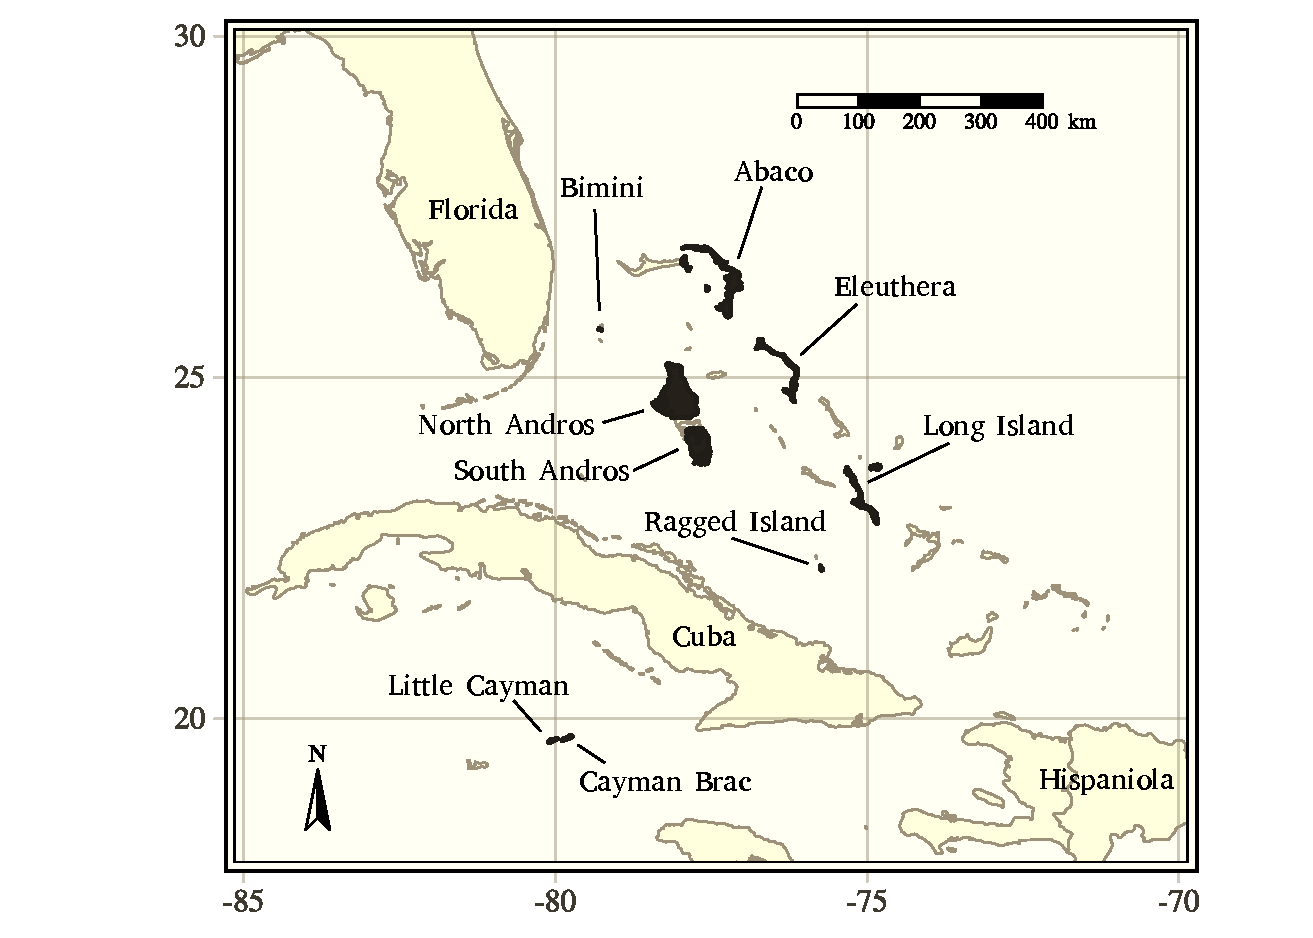
\includegraphics[width=0.8\textwidth]{../maps/map.pdf}
	\caption{Map of the West Indies with sampled islands highlighted in black.}
	\label{fig:map}
\end{figure}

% Boxplots and analyses of variance
\begin{sidewaysfigure}
	\centering
	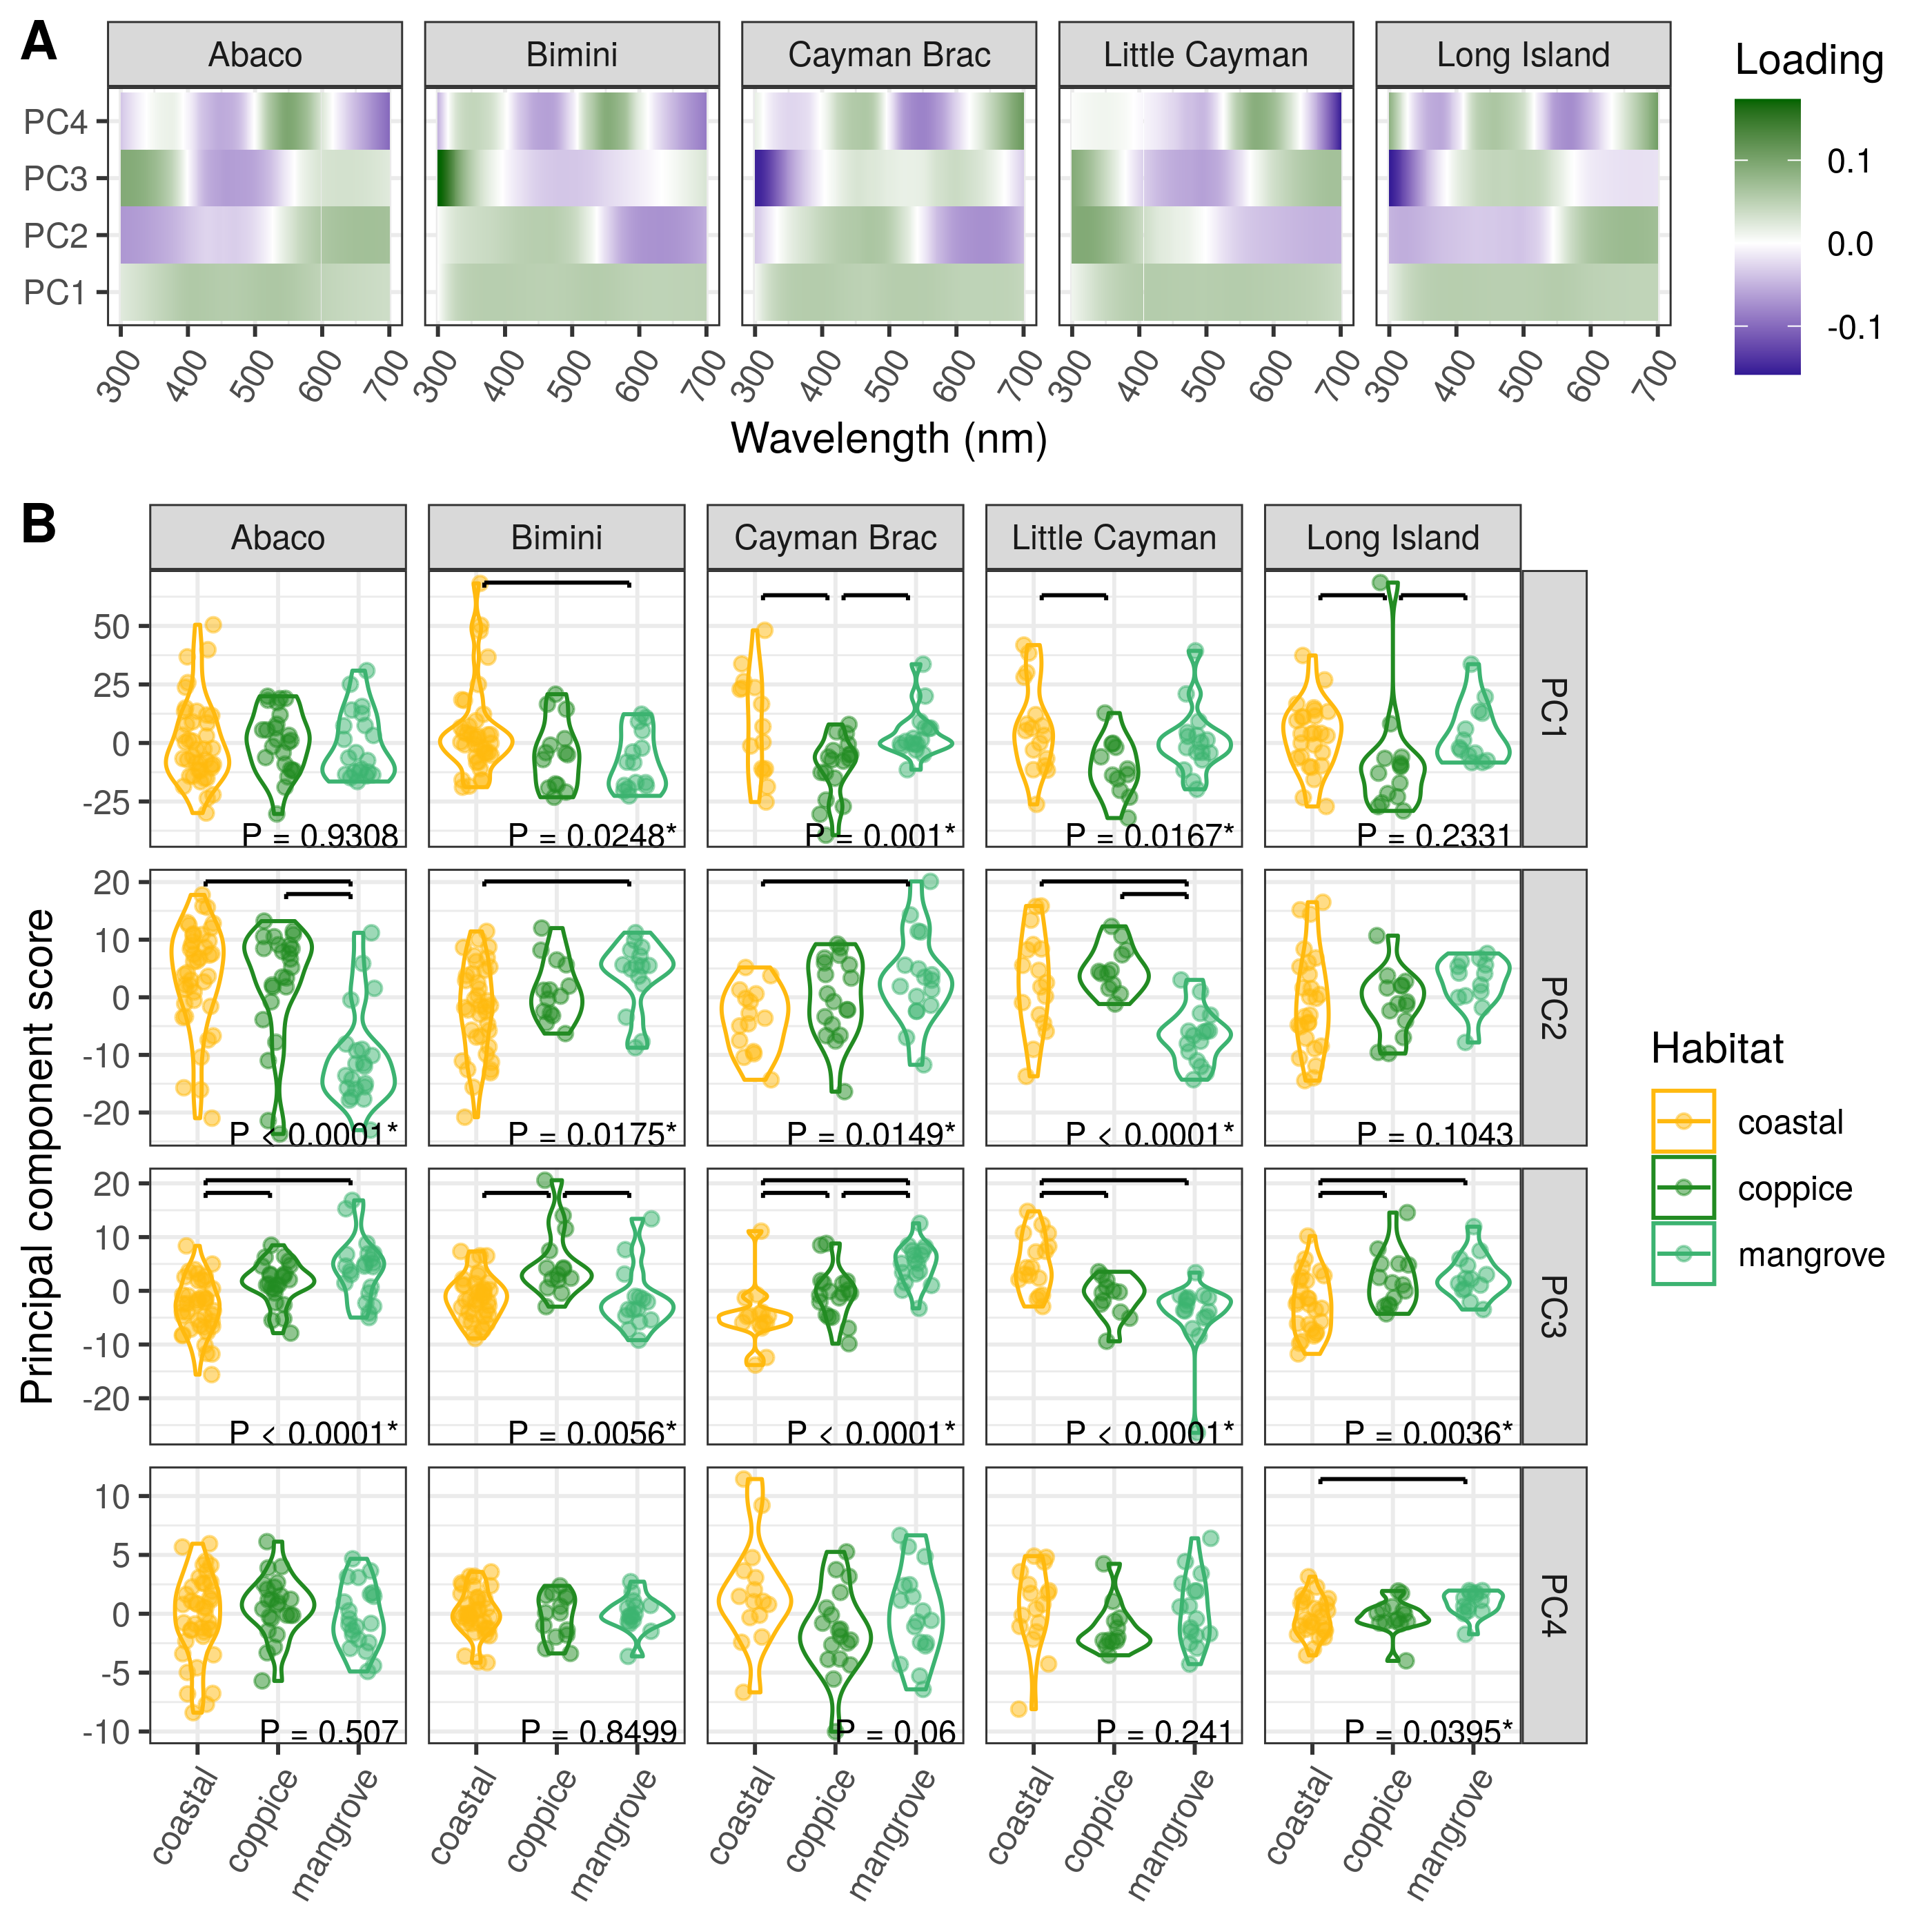
\includegraphics[width=18cm]{../analyses/07-ANOVA/figure_anova.png}
	\caption{Dewlap color variation between habitat-types across the most significant islands. (A) Mapping of reflectance at various wavelengths onto the principal components (loadings from the PCA rotation matrix). (B) Distribution of PC scores between habitats along the first four PCs on each island where significant between-habitat differences were detected using SVMs. P-values are reported for univariate ANOVA (or Kruskal-Wallis tests when applicable, see Methods). Post hoc significant differences at a 0.05 error rate are indicated with horizontal bars. *, P < 0.05.}
	\label{fig:anova}
\end{sidewaysfigure}

% Classification accuracy of SVMs
\begin{figure}[H]
    \centering
	\includegraphics[width=\textwidth]{"../analyses/04-machine learning/plots/classif_svm_pca"}
	\caption{SVM classification accuracy across islands based on principal component data. Histograms show accuracy distributions over 100 replicates for each five cross-validation bins per island. The dashed line is the density of a corresponding null binomial distribution, which would be expected under random guessing (testing sets with 20\% of the observations for each island and success probability of $1/3$). Inset plots show the corresponding average confusion matrices and represent the proportion of lizards from each habitat (columns) reassigned in each other habitat (rows), with an interpretation guide in the right panel. Binomial test P-values indicate deviations of the mean classification accuracy to the null distribution. *, P < 0.05.}
	\label{fig:classif-svm-pca}
\end{figure}


	\pagebreak

	\section*{Tables}

	\begin{table}
	\label{tab:anova}
	\caption{}
	\centering
	% ANOVA table
\begin{table}[H]
    \centering
    \caption{Analyses of variance (ANOVA) testing the effect of habitat-type on multiple response variables across the most significant islands according to the SVM classification (Figure \ref{fig:classif_svm_pca}). Best fit refers to the fitting method, i.e. OLS, ordinary least squares (favored when $\Delta$AICc $> 0$) or GLS, generalized least squares (favored when $\Delta$AICc $< 0$). AICc values are presented for the best-fitting model. df, degrees of freedom of the model; df$_{\mbox{LRT}}$, degrees of freedom of the likelihood ratio test (LRT) used to test the habitat effect; Log-lik., log-likelihood of the full model, i.e. including the habitat effect; $\chi^2$, likelihood-ratio between the full model and a null model excluding the habitat effect. *, P < 0.05; **, P < 0.01; ***, P < 0.001.}
    \begin{tabular}{lllrrrrrrll}
        \hline
        Island & Variable & Best fit & df & AICc & $\Delta$AICc & df$_{\mbox{LRT}}$ & Log-lik. & $\chi^2$ & P-value & \\
        \hline
        Abaco & PC1 & OLS & 4 & 710.40 & 2.16 & 2 & -356.96 & 0.14 & 0.9308 & \\
        Abaco & PC2 & OLS & 4 & 620.06 & 4.02 & 2 & -310.16 & 31.74 & < 0.0001 &  ***\\
        Abaco & PC3 & OLS & 4 & 517.80 & 2.01 & 2 & -257.18 & 27.37 & < 0.0001 &  ***\\
        Abaco & PC4 & OLS & 4 & 440.59 & 0.78 & 2 & -217.18 & 1.36 & 0.5070 &  \\
        Bimini & PC1 & OLS & 4 & 561.34 & 0.77 & 2 & -283.06 & 7.40 & 0.0248 &  *\\
        Bimini & PC2 & OLS & 4 & 448.06 & 1.29 & 2 & -223.77 & 8.09 & 0.0175 &  *\\
        Bimini & PC3 & GLS & 6 & 405.30 & -0.23 & 2 & -199.18 & 10.39 & 0.0056 &  **\\
        Bimini & PC4 & OLS & 4 & 274.15 & 3.54 & 2 & -132.74 & 0.33 & 0.8499 &  \\
        Cayman Brac & PC1 & GLS & 6 & 402.81 & -4.05 & 2 & -200.86 & 13.81 & 0.0010 &  **\\
        Cayman Brac & PC2 & OLS & 4 & 332.14 & 3.51 & 2 & -165.91 & 8.41 & 0.0149 &  *\\
        Cayman Brac & PC3 & OLS & 4 & 295.78 & 2.77 & 2 & -146.57 & 27.16 & < 0.0001 &  ***\\
        Cayman Brac & PC4 & OLS & 4 & 279.24 & 4.33 & 2 & -137.77 & 5.63 & 0.0600 &  \\
        Little Cayman & PC1 & OLS & 4 & 367.17 & 2.50 & 2 & -185.99 & 8.18 & 0.0167 &  *\\
        Little Cayman & PC2 & GLS & 6 & 287.61 & -3.61 & 2 & -140.46 & 29.76 & < 0.0001 &  ***\\
        Little Cayman & PC3 & OLS & 4 & 277.69 & 1.41 & 2 & -138.06 & 21.34 & < 0.0001 &  ***\\
        Little Cayman & PC4 & OLS & 4 & 226.70 & 2.53 & 2 & -110.74 & 2.85 & 0.2410 &  \\
        Long Island & PC1 & GLS & 6 & 442.34 & -2.09 & 2 & -221.16 & 2.91 & 0.2331 &  \\
        Long Island & PC2 & GLS & 6 & 351.37 & -3.08 & 2 & -172.57 & 4.52 & 0.1043 &  \\
        Long Island & PC3 & OLS & 4 & 322.06 & 3.67 & 2 & -159.98 & 11.24 & 0.0036 &  **\\
        Long Island & PC4 & OLS & 4 & 195.45 & 2.38 & 2 & -92.88 & 6.46 & 0.0395 &  *\\
        \hline
    \end{tabular}
    \label{tab:anova}
\end{table}
\end{table}





	\pagebreak

	\bibliographystyle{apalike}
	\bibliography{library.bib}
	
	\beginsupplement

	\pagebreak

	\section*{Appendix}
	
	Here we describe more precisely the patterns identified on each island.\\

On Abaco, dewlaps from the mangrove habitat were the best discriminated, while dewlaps from the beach scrub habitat were often mistaken for dewlaps from the coppice habitat (Fig. \ref{fig:Abaco}D). Importance analysis revealed that beach scrub and mangrove lizards mostly differed in reflectance in the ultraviolet (UV) end of the spectrum (below 400nm, Fig. \ref{fig:Abaco_supplement}F), where mangrove dewlaps had higher UV reflectance relative to beach scrub lizards, and coppice lizards had an intermediate UV reflectance between the two other habitats (Fig. \ref{fig:Abaco}B). Consistent with this, our analyses of variance detected significantly higher PC2 scores in mangrove lizards than in the two other habitats (Fig. \ref{fig:Abaco}E, Table \ref{tab:anova}), representing a higher UV-reflectance relative to red (Fig. \ref{fig:Abaco}C). Beach scrub lizards also scored higher on PC3 (Fig. \ref{fig:Abaco}E, Table \ref{tab:anova}), indicating less curvature of the reflectance profile and relatively higher reflectance at intermediate wavelengths (blue-to-yellow) than at the ends of the range (Fig. \ref{fig:Abaco}C). Differences were detected between sites both at large ($\sim$ 100km) and short ($<$ 1km) distances (Fig. \ref{fig:Abaco_supplement}G). Abaco was the only island where we detected significant spatial autocorrelation (Table \ref{tab:autocorrelation}), that is, sites that were closer geographically tended to have populations of lizards with more similar dewlap colors.\\

On Bimini, the random forests mostly correctly classified lizards from the coppice and mangrove habitats while often misclassifying lizards from the beach scrub habitat (Fig. \ref{fig:Bimini}D). Relatively flat importance profiles for beach scrub lizards suggested that brightness was used instead of a particular wavelength to identify some of the beach scrub dewlaps (Fig. \ref{fig:Bimini}F). Indeed, some beach scrub dewlaps were substantially brighter than the rest (Fig. \ref{fig:Bimini}B, C), a pattern that was captured by our analysis of variance along PC1 (i.e. brightness, Fig. \ref{fig:Bimini}C, E, Table \ref{tab:anova}). Coppice dewlaps had significantly higher PC2 scores than mangrove dewlaps (Fig. \ref{fig:Bimini}E), suggesting a higher curvature (higher UV and red reflectance than more intermediate wavelengths, Fig. \ref{fig:Bimini}C). For these two habitats the random forests were most sensitive to UV reflectance (Fig. \ref{fig:Bimini}F). Beach scrub dewlaps had higher PC3 scores than coppice dewlaps but it was not clear what properties of spectral shape this principal component mapped onto (Fig. \ref{fig:Bimini}C). On this island, the beach scrub and coppice habitats were separated by a few hundred meters, making this contrast the smallest geographical scale at which differences in coloration were found in our study (Fig. \ref{fig:Bimini}G).\\

On Cayman Brac, all three habitats could be well discriminated against each other (Fig. \ref{fig:CaymanBrac}D), with UV reflectance appearing to be an important variable differentiating beach scrub and mangrove dewlaps (Fig. \ref{fig:CaymanBrac}F). In contrast, coppice dewlaps had a relatively flat importance profile, suggesting that brightness made them more distinct rather than any particular wavelength (Fig. \ref{fig:CaymanBrac}F). Consistent with this, coppice dewlaps were significantly different from all other dewlaps along PC1 (Fig. \ref{fig:CaymanBrac}E, Table \ref{tab:anova}). At a distance between 2 and 3km (Fig. \ref{fig:CaymanBrac}G), dewlaps in the beach scrub habitat reflected more red light (as represented by PC2, Fig. \ref{fig:CaymanBrac}C, E) and more UV (as represented by PC3, along which coppice dewlaps were intermediate, Fig. \ref{fig:CaymanBrac}C, E) than in the mangrove habitat.\\

On Eleuthera, although random forests detected between-habitat differences in dewlap color, other approaches did not (Tables \ref{tab:ldas} and \ref{tab:ksvms}), suggesting that the differences may be small. On Eleuthera, beach scrub and mangrove dewlaps were guessed relatively correctly, but coppice dewlaps were more often mistaken for mangrove dewlaps (Fig. \ref{fig:Eleuthera}D). Mangrove dewlaps had lower PC2 scores than beach scrub dewlaps (Fig. \ref{fig:Eleuthera}E, indicating higher UV relative to red, Fig. \ref{fig:Eleuthera}C), and higher PC4 scores than coppice dewlaps (Fig. \ref{fig:Eleuthera}E, suggesting more reflectance profiles with more curvature, Fig. \ref{fig:Eleuthera}C). Random forests did not seem to consistently capture the wavelengths responsible for these differences (Fig. \ref{fig:Eleuthera}F).\\

Little Cayman was characterized by a better discrimination of mangrove lizards from the rest than between beach scrub and coppice lizards even though all habitats were relatively well discriminated (Fig. \ref{fig:LittleCayman}D). Mangrove dewlaps were most distinct with respect to their reflectance in short wavelengths (Fig. \ref{fig:LittleCayman}F), with significantly lower UV reflectance (as represented by PC2, Fig. \ref{fig:LittleCayman}C, E, Table \ref{tab:anova}). Beach scrub lizards were characterized by brighter dewlaps than coppice lizards (PC1), and also more convex curves, i.e. slightly higher UV and red reflectance (as represented by higher PC3 scores), than lizards from the other two habitats (Fig. \ref{fig:LittleCayman}C, E, Table \ref{tab:anova}).\\

On Long Island the three habitats were relatively well discriminated (Fig. \ref{fig:LongIsland}D). Importance profiles indicated that short wavelengths were used to discriminate between beach scrub and mangrove lizards (Fig. \ref{fig:LongIsland}F). Beach scrub lizards had more curved reflectance profiles than in the mangrove, with higher levels of UV and red reflectance relative to intermediate wavelengths (PC3, Fig. \ref{fig:LongIsland}C, E, Table \ref{tab:anova}). Coppice lizards were significantly darker than mangrove and beach scrub lizards (PC1, Fig. \ref{fig:LongIsland}C, E, Table \ref{tab:anova}).\\ 

On North Andros beach scrub and coppice dewlaps could be discriminated better against each other than with mangrove dewlaps (Fig. \ref{fig:NorthAndros}D), with importance profiles supporting UV-reflectance as a predictor of coppice lizards (Fig. \ref{fig:NorthAndros}F). Coppice lizards had less curved reflectance profiles than beach scrub and mangrove lizards (PC2), and beach scrub dewlaps had the lowest scores on PC4, which was difficult to interpret (Fig. \ref{fig:NorthAndros}C, E, Table \ref{tab:anova}).\\

Classification success was not significantly better than expected by chance on Ragged Island and South Andros (Table \ref{tab:randomforests}, \ref{tab:ldas}, \ref{tab:ksvms}) where nearly no habitat could be differentiated from any other based on reflectance.
	
	\pagebreak
	
	\section*{Supplementary Figures}
	
	% Map of each island
\begin{figure}[H]
\centering
	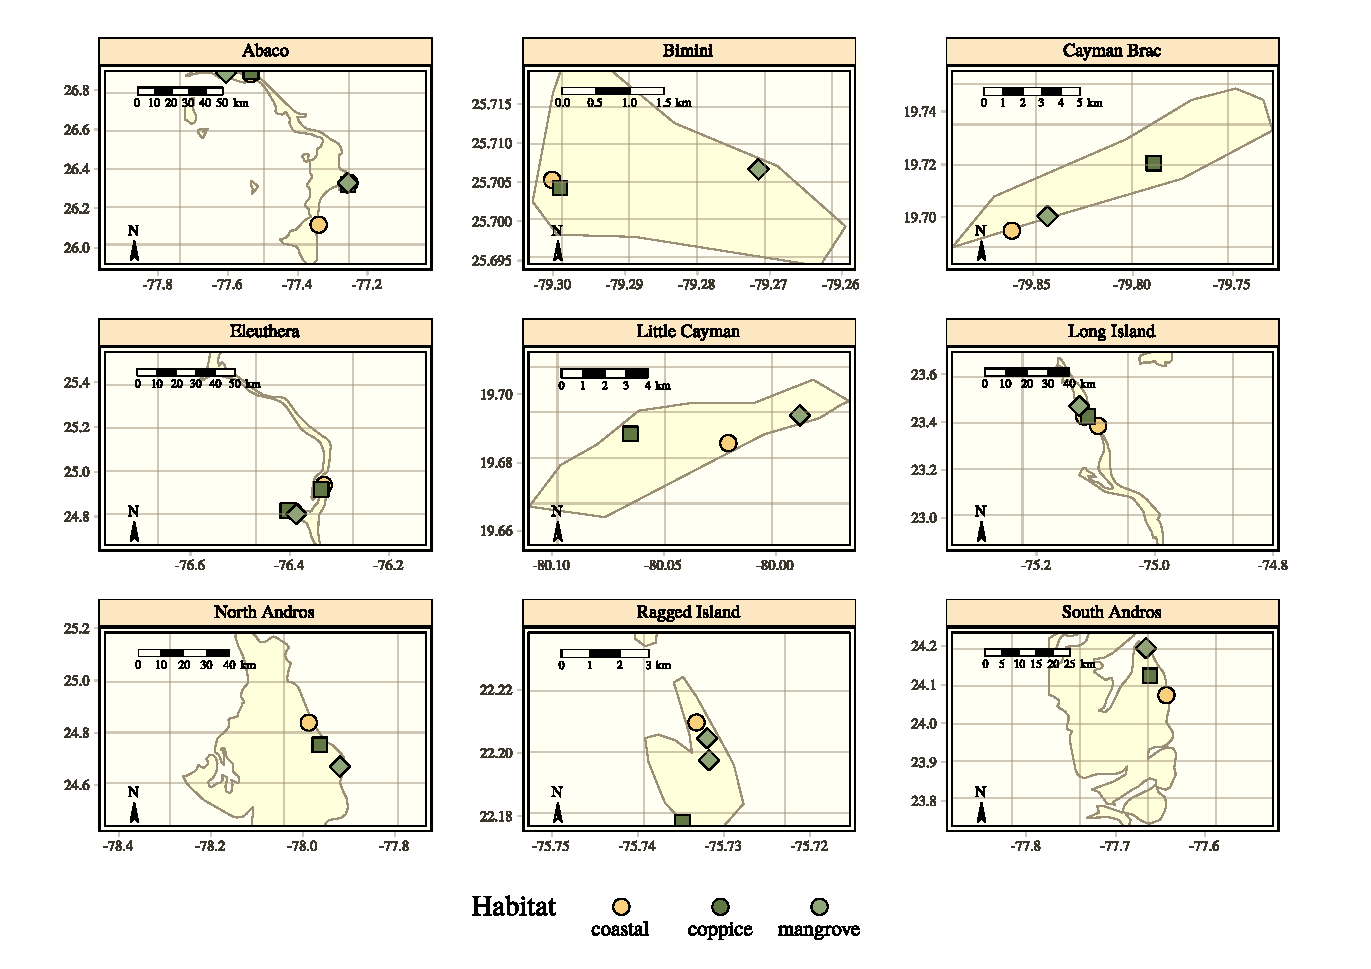
\includegraphics[width=\textwidth]{../maps/detailed_map.pdf}
	\caption{Map of the sampling sites and corresponding habitats across nine islands of the West Indies.}
	\label{supfig:map}
\end{figure}

\begin{figure}[H]
	\centering
	\includegraphics[width=0.8\textwidth]{"../analyses/03-PCA/figure_brightness"}
	\caption{Correlation between dewlap brightness (as measured by the mean reflectance from 300 to 700nm in wavelength) and PC1 score for each island. Pearson's squared correlation coefficients are reported. *, P < 0.05.}	
	\label{supfig:brightness}
\end{figure}

\begin{figure}[H]
	\centering
	\includegraphics[width=0.5\textwidth]{"../analyses/03-PCA/figure_brightness_pooled"}
	\caption{Correlation between dewlap brightness (as measured by the mean reflectance from 300 to 700nm in wavelength) and PC1 score across the whole archipelago. Pearson's squared correlation coefficient is reported. *, P < 0.05.}
	\label{supfig:brightness_pooled}
\end{figure}

\begin{figure}[H]
	\centering
	\includegraphics[width = \textwidth]{"../analyses/06-pooled/figure_pooled"}
	\caption{(A) Principal component scores and 5\% confidence ellipses across habitats for the whole archipelago. The principal component analysis was performed on reflectance data from all islands pooled together. (B) PCA rotation matrix showing the loadings of each wavelength from 300 to 700nm onto the principal components.}
	\label{supfig:pooled}
\end{figure}

% Reflectance curves
\begin{figure}[H]
	\centering
	\includegraphics[width=0.8\textwidth]{"../analyses/02-reflectance/figure_reflectance"}
	\caption{5-95th percentile range of lizard dewlap reflectance values (in \% of incoming light) across wavelengths for each island and each habitat.}
	\label{supfig:reflectance}
\end{figure}

\begin{figure}[H]
	\centering
	\includegraphics[width=0.8\textwidth]{"../analyses/04-machine learning/plots/classif_svm_pca_pooled"}
	\caption{Archipelago-wide SVM classification accuracy based on principal component data. Machines were trained on individual dewlaps regardless of island identity. The histogram shows the accuracy distribution over 100 replicates for each five cross-validation bins. The legend is the same as in Figure \ref{fig:classif-svm-pca}.}
	\label{supfig:classif-svm-pca-pooled}
\end{figure}

\begin{figure}[H]
	\centering
	\includegraphics[width=0.8\textwidth]{"../analyses/04-machine learning/plots/classif_svm_refl_pooled"}
	\caption{Archipelago-wide SVM classification accuracy based on reflectance data at 50nm-intervals in wavelength (see Methods). Machines were trained on individual dewlaps regardless of island identity. The histogram shows the accuracy distribution over 100 replicates for each five cross-validation bins. The legend is the same as in Figure \ref{fig:classif-svm-pca}.}
	\label{supfig:classif-svm-refl-pooled}
\end{figure}

\begin{figure}[H]
	\centering
	\includegraphics[width=0.4\textwidth]{"../analyses/04-machine learning/plots/importance_svm_pca_pooled"}
	\caption{Sensitivity analyses of the different input variables in the archipelago-wide SVM classification on principal component data (Figure \ref{supfig:classif-svm-pca-pooled}), with relative importance computed for every machine.}
	\label{supfig:importance-svm-pca-pooled}
\end{figure}

\begin{figure}[H]
	\centering
	\includegraphics[width=0.6\textwidth]{"../analyses/04-machine learning/plots/importance_svm_refl_pooled"}
	\caption{Sensitivity analyses of the different input variables in the archipelago-wide SVM classification on reflectance data at 50nm-intervals in wavelength (Figure \ref{supfig:classif-svm-refl-pooled}), with relative importance computed for every machine.}
	\label{supfig:importance-svm-refl-pooled}
\end{figure}

\begin{figure}[H]
	\centering
	\includegraphics[width=0.8\textwidth]{"../analyses/04-machine learning/plots/classif_lda_pca_pooled"}
	\caption{Archipelago-wide LDA classification accuracy based on principal component data. Machines were trained on individual dewlaps regardless of island identity. The histogram shows the accuracy distribution over 100 replicates for each five cross-validation bins. The legend is the same as in Figure \ref{fig:classif-svm-pca}.}
	\label{supfig:classif-lda-pca-pooled}
\end{figure}

\begin{figure}[H]
	\centering
	\includegraphics[width=0.8\textwidth]{"../analyses/04-machine learning/plots/classif_lda_refl_pooled"}
	\caption{Archipelago-wide LDA classification accuracy based on reflectance data at 50nm-intervals in wavelength (see Methods). Machines were trained on individual dewlaps regardless of island identity. The histogram shows the accuracy distribution over 100 replicates for each five cross-validation bins. The legend is the same as in Figure \ref{fig:classif-svm-pca}.}
	\label{supfig:classif-lda-refl-pooled}
\end{figure}

\begin{figure}[H]
	\centering
	\includegraphics[width=\textwidth]{"../analyses/04-machine learning/plots/classif_lda_pca"}
	\caption{LDA classification accuracy across islands based on principal component data. Histograms show accuracy distributions over 100 replicates for each five cross-validation bins per island. The legend is the same as in Figure \ref{fig:classif-svm-pca}.}
	\label{supfig:classif-lda-pca}
\end{figure}

\begin{figure}[H]
	\centering
	\includegraphics[width=\textwidth]{"../analyses/04-machine learning/plots/classif_svm_refl"}
	\caption{SVM classification accuracy across islands based on reflectance data at 50nm-intervals in wavelength (see Methods). Histograms show accuracy distributions over 100 replicates for each five cross-validation bins per island. The legend is the same as in Figure \ref{fig:classif-svm-pca}.}
	\label{supfig:classif-svm-refl}
\end{figure}

\begin{figure}[H]
	\centering
	\includegraphics[width=\textwidth]{"../analyses/04-machine learning/plots/classif_lda_refl"}
	\caption{LDA classification accuracy across islands based on reflectance data at 50nm-intervals in wavelength (see Methods). Histograms show accuracy distributions over 100 replicates for each five cross-validation bins per island. The legend is the same as in Figure \ref{fig:classif-svm-pca}.}
	\label{supfig:classif-lda-refl}
\end{figure}

\begin{figure}[H]
	\centering
	\includegraphics[width=0.8\textwidth]{"../analyses/04-machine learning/plots/importance_svm_pca"}
	\caption{Sensitivity analyses of the different input variables in the within-island SVM classification on principal component data (Figure \ref{supfig:classif-svm-pca}), with relative importance computed for every machine.}
	\label{supfig:importance-svm-pca}
\end{figure}

\begin{figure}[H]
	\centering
	\includegraphics[width=0.8\textwidth]{"../analyses/04-machine learning/plots/importance_lda_pca"}
	\caption{Sensitivity analyses of the different input variables in the within-island LDA classification on principal component data (Figure \ref{supfig:classif-lda-pca}), with relative importance computed for every machine.}
	\label{supfig:importance-lda-pca}
\end{figure}

\begin{figure}[H]
	\centering
	\includegraphics[width=0.8\textwidth]{"../analyses/04-machine learning/plots/importance_svm_pca"}
	\caption{Sensitivity analyses of the different input variables in the archipelago-wide SVM classification on reflectance at 50nm-intervals in wavelength (Figure \ref{supfig:classif-svm-refl}), with relative importance computed for every machine.}
	\label{supfig:importance-svm-refl}
\end{figure}

\begin{figure}[H]
	\centering
	\includegraphics[width=0.8\textwidth]{"../analyses/04-machine learning/plots/importance_lda_pca"}
	\caption{Sensitivity analyses of the different input variables in the archipelago-wide LDA classification on reflectance at 50nm-intervals in wavelength (Figure \ref{supfig:classif-lda-refl}), with relative importance computed for every machine.}
	\label{supfig:importance-lda-refl}
\end{figure}

\begin{figure}[H]
	\centering
	\includegraphics[width=\textwidth]{"../analyses/10-distances/figure_distances2"}
	\caption{Spatial scale of between-habitat differences in dewlap coloration. For each variable and each pair of habitats where significant differences were detected (Figure \ref{fig:anova}), we performed multiple post hoc pairwise comparisons between the sites involved (Figure \ref{supfig:map}, Table \ref{suptab:sites}), using nonparametric Wilcoxon-Mann-Whitney tests. Here we report, for each pair of habitats, the distances between sites that significantly differed in dewlap coloration at an error rate of 0.05 (P-values corrected with the Benjamini-Hochberg procedure for multiple testing).}
	\label{supfig:distances}
\end{figure}

\begin{figure}[H]
	\centering
	\includegraphics[width=0.7\textwidth]{"../analyses/09-parallelism/figure_contrasts"}
	\caption{Test of parallel divergence between islands. Differences in habitat-means, or contrasts, are shown for two pairs of habitats for each principal component on each island, rescaled so the standard deviation of the means along each principal component is one. The contrasts represent the patterns of between-habtiat variation on each island, for a given principal component. The absence of clustering of islands by variable indicates that islands differ in their between-habitat divergence patterns. This is confirmed by a non-significant MANOVA test of the between versus within-variable variance in contrasts.}
	\label{supfig:contrasts}
\end{figure}
	
	\pagebreak
	
	\section*{Supplementary Tables}
	
	\begin{table}[H]	
	\caption{Number of lizards sampled in each habitat on each island.}
	\centering
	
\begin{tabular}{l|r|r|r}
\hline
  & coastal & coppice & mangrove\\
\hline
Abaco & 41 & 24 & 21\\
\hline
Bimini & 38 & 14 & 15\\
\hline
Cayman Brac & 15 & 18 & 17\\
\hline
Eleuthera & 22 & 25 & 9\\
\hline
Little Cayman & 17 & 12 & 16\\
\hline
Long Island & 26 & 14 & 13\\
\hline
North Andros & 9 & 9 & 10\\
\hline
Ragged Island & 18 & 15 & 17\\
\hline
South Andros & 10 & 9 & 12\\
\hline
\end{tabular}

	\label{suptab:counts}
\end{table}

\begin{table}[H]
	\caption{Locations of the sampling sites across islands, with mean principal component scores per site.}
	\centering
	
\begin{tabular}{lrrlrrrr}
\toprule
Island & Longitude & Latitude & Habitat & PC1 & PC2 & PC3 & PC4\\
\midrule
Abaco & -77.7256 & 26.9083 & mangrove & -5.4905 & 1.3541 & -0.4741 & 0.0083\\
Abaco & -77.5800 & 26.9020 & coastal & 1.8633 & 0.0365 & -0.4475 & 0.0033\\
Abaco & -77.5763 & 26.9128 & coppice & -1.6738 & -1.7793 & -0.0499 & 0.0012\\
Abaco & -77.1784 & 26.1045 & coastal & 1.1863 & 2.0408 & -0.3468 & 0.0022\\
Abaco & -77.0055 & 26.3254 & mangrove & -9.0319 & -2.7460 & 0.4687 & 0.0077\\
Abaco & -77.0039 & 26.3170 & coppice & 0.9967 & 0.5161 & -0.0267 & -0.0118\\
Abaco & -76.9968 & 26.3260 & coastal & 7.6077 & 0.3186 & 0.1771 & -0.0008\\
Bimini & -79.3022 & 25.5859 & coastal & 5.7537 & -0.1593 & -0.2505 & 0.0001\\
Bimini & -79.3014 & 25.7052 & coastal & -3.1822 & 1.6617 & -0.0460 & 0.0024\\
Bimini & -79.3002 & 25.7042 & coppice & -1.3514 & -3.8786 & 0.1027 & -0.0027\\
Bimini & -79.2709 & 25.7066 & mangrove & 3.3656 & 0.6244 & 0.1569 & -0.0021\\
Cayman Brac & -79.8627 & 19.6878 & coastal & 6.6606 & -2.5670 & 0.0166 & -0.0007\\
Cayman Brac & -79.8441 & 19.6949 & mangrove & -1.0914 & 4.3607 & 0.0855 & 0.0001\\
Cayman Brac & -79.7887 & 19.7209 & coppice & -4.5197 & -1.9793 & -0.0946 & 0.0004\\
Eleuthera & -76.3347 & 24.8146 & coppice & 3.2669 & -1.2404 & 0.1018 & -0.0085\\
Eleuthera & -76.3058 & 24.8127 & coastal & 0.4216 & -3.5133 & -0.0567 & 0.0009\\
Eleuthera & -76.2901 & 24.7981 & mangrove & 2.1881 & 0.7517 & 0.3957 & -0.0055\\
Eleuthera & -76.1616 & 24.9129 & coppice & -1.9136 & 1.0868 & -0.4978 & -0.0092\\
Eleuthera & -76.1492 & 24.9335 & coastal & -3.1863 & 2.4270 & 0.1881 & 0.0218\\
Little Cayman & -80.0660 & 19.6906 & coppice & 0.8021 & -1.9569 & -0.0760 & -0.0068\\
Little Cayman & -80.0205 & 19.6865 & coastal & -6.6917 & -1.2615 & 0.0659 & 0.0057\\
Little Cayman & -79.9871 & 19.6986 & mangrove & 6.5083 & 2.8079 & -0.0129 & -0.0010\\
Long Island & -75.2299 & 23.4740 & mangrove & -1.2873 & 1.9371 & -0.1880 & -0.0029\\
Long Island & -75.2063 & 23.4282 & coastal & 2.3686 & -0.9033 & 0.0215 & 0.0096\\
Long Island & -75.1884 & 23.4292 & coppice & -4.6266 & 0.5060 & 0.1049 & -0.0070\\
Long Island & -75.1408 & 23.3883 & coastal & 3.6139 & -1.4521 & 0.0475 & 0.0025\\
North Andros & -77.8908 & 24.8391 & coastal & -2.1881 & -1.1236 & 0.0397 & -0.0060\\
North Andros & -77.8428 & 24.7516 & coppice & -1.8115 & 0.0012 & -0.1678 & 0.0024\\
North Andros & -77.7540 & 24.6644 & mangrove & 3.5997 & 1.0101 & 0.1153 & 0.0033\\
Ragged Island & -75.7364 & 22.1768 & coppice & 3.2851 & -0.3274 & 0.1911 & -0.0013\\
Ragged Island & -75.7314 & 22.2097 & coastal & -0.6412 & -0.8878 & -0.1293 & -0.0033\\
Ragged Island & -75.7276 & 22.2045 & mangrove & -2.9188 & 1.5792 & -0.0034 & 0.0099\\
Ragged Island & -75.7270 & 22.1973 & mangrove & -1.2210 & 0.7285 & -0.0721 & -0.0028\\
South Andros & -77.6050 & 24.2027 & mangrove & -3.9253 & 0.4734 & 0.0477 & -0.0005\\
South Andros & -77.5936 & 24.1289 & coppice & 6.1152 & -0.4925 & 0.0349 & 0.0012\\
South Andros & -77.5453 & 24.0764 & coastal & -0.7933 & -0.1248 & -0.0887 & -0.0004\\
\bottomrule
\end{tabular}

	\label{suptab:sites}
\end{table}

\begin{table}[H]
	\caption{Proportion of variance explained by the first four principal components on each island, as well as across the whole archipelago.}
	\centering
	
\begin{tabular}{l|r|r|r|r|r}
\hline
island & PC1 & PC2 & PC3 & PC4 & total\\
\hline
Abaco & 0.400 & 0.279 & 0.147 & 0.079 & 0.906\\
\hline
Bimini & 0.502 & 0.208 & 0.160 & 0.051 & 0.921\\
\hline
Cayman Brac & 0.438 & 0.190 & 0.155 & 0.105 & 0.888\\
\hline
Eleuthera & 0.490 & 0.233 & 0.138 & 0.066 & 0.926\\
\hline
Little Cayman & 0.441 & 0.212 & 0.176 & 0.078 & 0.907\\
\hline
Long Island & 0.515 & 0.205 & 0.161 & 0.043 & 0.925\\
\hline
North Andros & 0.560 & 0.170 & 0.152 & 0.054 & 0.937\\
\hline
Ragged Island & 0.483 & 0.226 & 0.127 & 0.072 & 0.907\\
\hline
South Andros & 0.488 & 0.247 & 0.146 & 0.067 & 0.948\\
\hline
Archipelago & 0.473 & 0.197 & 0.164 & 0.079 & 0.913\\
\hline
\end{tabular}

	\label{suptab:pcavariances}
\end{table}

\begin{table}[H]
	\caption{Pearson's correlation test between dewlap brightness, as measured by the average reflectance between 300 and 700nm in wavelength, and PC1 scores, for all islands and across the whole archipelago. ***, P < 0.001.}
	\centering
	
\begin{tabular}{l|r|l|l}
\hline
island & r2 & pvalue & \\
\hline
Abaco & 0.908 & < 0.0001 & ***\\
\hline
Bimini & 0.999 & < 0.0001 & ***\\
\hline
Cayman Brac & 0.987 & < 0.0001 & ***\\
\hline
Eleuthera & 0.963 & < 0.0001 & ***\\
\hline
Little Cayman & 0.965 & < 0.0001 & ***\\
\hline
Long Island & 0.986 & < 0.0001 & ***\\
\hline
North Andros & 0.994 & < 0.0001 & ***\\
\hline
Ragged Island & 0.978 & < 0.0001 & ***\\
\hline
South Andros & 0.979 & < 0.0001 & ***\\
\hline
Archipelago & 0.976 & < 0.0001 & ***\\
\hline
\end{tabular}

	\label{suptab:brightness}
\end{table}

\begin{table}[H]
	\caption{Henze-Zirkler's test of multivariate normality, performed on principal components in each habitat and on each island. HZ, test statistic. *, P < 0.05; **, P < 0.01; ***, P < 0.001.}
	\centering
	
\begin{tabular}{llrrl}
\toprule
island & habitat & HZ & pvalue & signif\\
\midrule
Abaco & coastal & 1.10 & 0.0027 & **\\
Abaco & coppice & 1.07 & 0.0022 & **\\
Abaco & mangrove & 1.06 & 0.0023 & **\\
Bimini & coastal & 1.28 & 0.0001 & ***\\
Bimini & coppice & 0.85 & 0.0482 & *\\
\addlinespace
Bimini & mangrove & 1.19 & 0.0001 & ***\\
Cayman Brac & coastal & 0.65 & 0.5311 & \\
Cayman Brac & coppice & 0.70 & 0.3940 & \\
Cayman Brac & mangrove & 0.66 & 0.5357 & \\
Eleuthera & coastal & 1.61 & 0.0000 & ***\\
\addlinespace
Eleuthera & coppice & 1.48 & 0.0000 & ***\\
Eleuthera & mangrove & 0.73 & 0.1423 & \\
Little Cayman & coastal & 0.62 & 0.6599 & \\
Little Cayman & coppice & 0.64 & 0.4867 & \\
Little Cayman & mangrove & 0.87 & 0.0413 & *\\
\addlinespace
Long Island & coastal & 0.82 & 0.1468 & \\
Long Island & coppice & 0.92 & 0.0150 & *\\
Long Island & mangrove & 0.77 & 0.1289 & \\
North Andros & coastal & 0.66 & 0.3174 & \\
North Andros & coppice & 0.76 & 0.0900 & \\
\addlinespace
North Andros & mangrove & 0.67 & 0.3185 & \\
Ragged Island & coastal & 0.76 & 0.2268 & \\
Ragged Island & coppice & 0.80 & 0.1115 & \\
Ragged Island & mangrove & 0.54 & 0.9022 & \\
South Andros & coastal & 0.66 & 0.3451 & \\
\addlinespace
South Andros & coppice & 0.66 & 0.3154 & \\
South Andros & mangrove & 0.91 & 0.0144 & *\\
\bottomrule
\end{tabular}

	\label{suptab:multinorm}
\end{table}

\begin{table}[H]
	\caption{Box's M-test of homogeneity of covariance matrices across habitats on each island. $\chi^2$, test statistic. *, P < 0.05; **, P < 0.01; ***, P < 0.001.}
	\centering
	
\begin{tabular}{lrrrl}
\toprule
Island & $\chi^2$ & df & $P$ & \\
\midrule
Abaco & 47.1 & 20 & 0.0006 & ***\\
Bimini & 36.0 & 20 & 0.0152 & *\\
Cayman Brac & 36.9 & 20 & 0.0120 & *\\
Eleuthera & 44.6 & 20 & 0.0013 & **\\
Little Cayman & 32.8 & 20 & 0.0356 & *\\
Long Island & 56.2 & 20 & 0.0000 & ***\\
North Andros & 33.7 & 20 & 0.0283 & *\\
Ragged Island & 29.3 & 20 & 0.0824 & \\
South Andros & 46.5 & 20 & 0.0007 & ***\\
\bottomrule
\end{tabular}

	\label{suptab:covariance}
\end{table}

\begin{table}[H]
	\caption{Shapiro-Wilk's test of univariate normality performed on each island where significant differences were detected by SVM classification, in each habitat where deviations from multivariate normality were detected. $W$, test statistic. *, P < 0.05; **, P < 0.01; ***, P < 0.001.}
	\centering
	
\begin{tabular}{lllrrl}
\toprule
Island & Habitat & Variable & $W$ & $P$ & \\
\midrule
Abaco & coastal & PC1 & 0.954 & 0.0941 & \\
Abaco & coastal & PC2 & 0.927 & 0.0112 & *\\
Abaco & coastal & PC3 & 0.973 & 0.4228 & \\
Abaco & coastal & PC4 & 0.955 & 0.1027 & \\
Abaco & coppice & PC1 & 0.970 & 0.6776 & \\
Abaco & coppice & PC2 & 0.816 & 0.0005 & ***\\
Abaco & coppice & PC3 & 0.930 & 0.0976 & \\
Abaco & coppice & PC4 & 0.941 & 0.1711 & \\
Abaco & mangrove & PC1 & 0.881 & 0.0155 & *\\
Abaco & mangrove & PC2 & 0.869 & 0.0093 & **\\
Abaco & mangrove & PC3 & 0.986 & 0.9873 & \\
Abaco & mangrove & PC4 & 0.939 & 0.2044 & \\
Bimini & coastal & PC1 & 0.821 & 0.0000 & ***\\
Bimini & coastal & PC2 & 0.960 & 0.1854 & \\
Bimini & coastal & PC3 & 0.856 & 0.0002 & ***\\
Bimini & coastal & PC4 & 0.945 & 0.0611 & \\
Bimini & coppice & PC1 & 0.911 & 0.1648 & \\
Bimini & coppice & PC2 & 0.958 & 0.6927 & \\
Bimini & coppice & PC3 & 0.953 & 0.6146 & \\
Bimini & coppice & PC4 & 0.971 & 0.8953 & \\
Bimini & mangrove & PC1 & 0.884 & 0.0536 & \\
Bimini & mangrove & PC2 & 0.976 & 0.9363 & \\
Bimini & mangrove & PC3 & 0.982 & 0.9805 & \\
Bimini & mangrove & PC4 & 0.975 & 0.9232 & \\
Eleuthera & coastal & PC1 & 0.909 & 0.0461 & *\\
Eleuthera & coastal & PC2 & 0.886 & 0.0157 & *\\
Eleuthera & coastal & PC3 & 0.906 & 0.0390 & *\\
Eleuthera & coastal & PC4 & 0.962 & 0.5293 & \\
Eleuthera & coppice & PC1 & 0.922 & 0.0567 & \\
Eleuthera & coppice & PC2 & 0.954 & 0.3055 & \\
Eleuthera & coppice & PC3 & 0.781 & 0.0001 & ***\\
Eleuthera & coppice & PC4 & 0.901 & 0.0188 & *\\
Little Cayman & mangrove & PC1 & 0.907 & 0.1024 & \\
Little Cayman & mangrove & PC2 & 0.904 & 0.0924 & \\
Little Cayman & mangrove & PC3 & 0.739 & 0.0005 & ***\\
Little Cayman & mangrove & PC4 & 0.973 & 0.8802 & \\
Long Island & coppice & PC1 & 0.686 & 0.0003 & ***\\
Long Island & coppice & PC2 & 0.848 & 0.0210 & *\\
Long Island & coppice & PC3 & 0.931 & 0.3188 & \\
Long Island & coppice & PC4 & 0.904 & 0.1280 & \\
South Andros & mangrove & PC1 & 0.787 & 0.0067 & **\\
South Andros & mangrove & PC2 & 0.861 & 0.0500 & *\\
South Andros & mangrove & PC3 & 0.697 & 0.0008 & ***\\
South Andros & mangrove & PC4 & 0.950 & 0.6411 & \\
\bottomrule
\end{tabular}

	\label{suptab:normality}
\end{table}

\begin{table}[H]
	\caption{Univariate ANOVAs performed on each principal component across the whole archipelago. Legend is the same as for Table \ref{tab:anova}, except that best fitting models 3 and 4 refer to the mixed effect equivalents to the OLS and GLS model, with island as a random effect (see Methods).}
	\centering
	
\begin{tabular}{lrrrrrrrrrl}
\toprule
variable & best\_fit & df\_model & AICc & dAICc & AICcw & df\_LRT & loglik & lratio & pvalue & signif\\
\midrule
PC1 & 3 & 5 & 3749.9 & -228.3 & 0.613 & 2 & -1874.7 & 8.69 & 0.0130 & *\\
PC2 & 4 & 7 & 3002.2 & -162.3 & 0.976 & 2 & -1496.2 & 17.76 & 0.0001 & ***\\
PC3 & 4 & 7 & 2826.3 & -175.4 & 0.968 & 2 & -1407.8 & 7.03 & 0.0298 & *\\
PC4 & 4 & 7 & 2015.7 & -305.8 & 0.519 & 2 & -1000.1 & 0.47 & 0.7914 & \\
\bottomrule
\end{tabular}

	\label{suptab:anova-pooled}
\end{table}

\begin{table}[H]
	\caption{Mean SVM classification accuracy per island, over all replicates and cross-validation bins. $N$, number of observations per island; $p_{\mbox{test}}$, proportion of the data sampled to form the training set; $n_{\mbox{test}}$, number of observations in the testing set. P-values indicate deviations from the expected null binomial distribution, with $n_{\mbox{test}}$ events per island and random guess success probability $1/3$. *, P < 0.05, **, P < 0.01, ***, P < 0.001.}
	\centering
	
\begin{tabular}{lrrrrrl}
\toprule
Island & Accuracy & $N$ & $p_{\mbox{test}}$ & $n_{\mbox{test}}$ & $P$ & \\
\midrule
Abaco & 0.612 & 86 & 0.2 & 17 & 0.0080 & **\\
Bimini & 0.547 & 67 & 0.2 & 13 & 0.0347 & *\\
Cayman Brac & 0.721 & 50 & 0.2 & 10 & 0.0034 & **\\
Eleuthera & 0.437 & 56 & 0.2 & 11 & 0.2890 & \\
Little Cayman & 0.734 & 45 & 0.2 & 9 & 0.0083 & **\\
Long Island & 0.651 & 53 & 0.2 & 10 & 0.0197 & *\\
North Andros & 0.453 & 28 & 0.2 & 5 & 0.2099 & \\
Ragged Island & 0.364 & 50 & 0.2 & 10 & 0.4407 & \\
South Andros & 0.600 & 31 & 0.2 & 6 & 0.1001 & \\
\bottomrule
\end{tabular}
	
	\label{suptab:classif-svm-pca}
\end{table}

\begin{table}[H]
	\caption{Results of nonparametric Kruskal-Wallis tests performed on each variable on each island where deviations from normality were detected.}
	\centering
	
\begin{tabular}{llrrrl}
\toprule
island & variable & chisq & df & pvalue & signif\\
\midrule
Abaco & PC1 & 0.74 & 2 & 0.6924 & \\
Abaco & PC2 & 23.13 & 2 & 0.0000 & ***\\
Bimini & PC1 & 7.38 & 2 & 0.0250 & *\\
Bimini & PC3 & 15.17 & 2 & 0.0005 & ***\\
Little Cayman & PC3 & 19.95 & 2 & 0.0000 & ***\\
\addlinespace
Long Island & PC1 & 10.98 & 2 & 0.0041 & **\\
Long Island & PC2 & 4.02 & 2 & 0.1339 & \\
\bottomrule
\end{tabular}

	\label{suptab:kruskal}
\end{table}

\begin{table}[H]
	\caption{Individual-based permutation tests of spatial autocorrelation within islands. P-values were computed from 1,000 permutations of individual site-labels. Pearson's coefficient $r$ measures the correlation between distances in color space and geodesic distances among the sites. $N$, number of sites. *, P < 0.05.}
	\centering
	
\begin{tabular}{lrrrl}
\toprule
Island & $r$ & $P$ & $N$ & \\
\midrule
Abaco & -0.213 & 0.817 & 7 & \\
Bimini & 0.044 & 0.510 & 4 & \\
Cayman Brac & -0.010 & 0.465 & 3 & \\
Eleuthera & 0.816 & 0.015 & 5 & *\\
Little Cayman & -0.688 & 0.684 & 3 & \\
Long Island & -0.189 & 0.579 & 4 & \\
North Andros & 0.730 & 0.199 & 3 & \\
Ragged Island & 0.706 & 0.114 & 4 & \\
South Andros & -0.852 & 0.776 & 3 & \\
\bottomrule
\end{tabular}

	\label{suptab:autocor}
\end{table}

\end{document}

